\documentclass[11pt,a4paper]{article}
\usepackage[margin=2.5cm]{geometry}
\usepackage{amsmath,amssymb}
\usepackage{graphicx}
\usepackage{booktabs}
\usepackage{hyperref}
\usepackage{xcolor}
\usepackage{enumitem}
\usepackage{caption}
\usepackage{subcaption}
\usepackage{listings}
\usepackage{float}

\hypersetup{colorlinks=true, linkcolor=blue, citecolor=blue, urlcolor=blue}

\lstset{
  basicstyle=\ttfamily\small,
  keywordstyle=\color{blue},
  commentstyle=\color{gray},
  breaklines=true,
  frame=single,
  backgroundcolor=\color{gray!8}
}

\title{\textbf{Deep Q-Networks on Atari}\\
       \large Reinforcement Learning Homework — BIU 2026}
\author{Aviv Weidenfeld \and Shani Or Levy}
\date{May 2026}

\begin{document}
\maketitle
\tableofcontents
\newpage

%% ─────────────────────────────────────────────────────────────────────────────
\section{Game Choice}

We trained the DQN agent on \textbf{Alien} (\texttt{ALE/Alien-v5}).

\subsection*{Why Alien?}
Alien is a moderately complex Atari game with a well-defined reward signal (shooting aliens,
collecting power pellets, progressing through mazes). It has a meaningful gap between random
and trained agent performance, making it an informative benchmark.

\begin{center}
\begin{tabular}{lrr}
\toprule
\textbf{Threshold} & \textbf{Score} & \textbf{Status} \\
\midrule
Random agent (minimum must) & 227.8 & \textcolor{green!60!black}{$\checkmark$ Passed} \\
Good grade (best linear agent) & 950.0 & \textcolor{green!60!black}{$\checkmark$ Passed — avg 3170.6} \\
Bonus grade (DQN paper score) & 3000.0 & \textcolor{green!60!black}{$\checkmark$ Passed — avg 3170.6} \\
\bottomrule
\end{tabular}
\end{center}

%% ─────────────────────────────────────────────────────────────────────────────
\section{Preprocessing}

We follow the preprocessing from Mnih et al.\ (2013) closely:

\begin{enumerate}
  \item \textbf{Grayscale conversion}: Each RGB frame $(210 \times 160 \times 3)$ is
        converted to grayscale using \texttt{cv2.COLOR\_RGB2GRAY}.

  \item \textbf{Resize and crop}: The grayscale frame is resized to $84 \times 110$
        using \texttt{cv2.INTER\_AREA} interpolation, then cropped to $84 \times 84$
        by removing 18 pixels from the top and 8 from the bottom (rows 18--102).

  \item \textbf{Frame skipping}: The agent repeats each selected action for 4 raw
        environment steps (\texttt{frame\_skip=4}), accumulating reward across them.
        This matches the paper's action repetition.

  \item \textbf{Max-pooling over last 2 frames}: To eliminate sprite flickering
        (a known ALE artefact), the observation fed to the network is the pixel-wise
        maximum of the last 2 frames within each skip block.

  \item \textbf{Frame stacking}: The last 4 preprocessed frames are stacked into a
        $(4 \times 84 \times 84)$ tensor, giving the network temporal context.
        Frames are stored as \texttt{uint8} in the replay buffer and cast to
        \texttt{float32} in $[0,1]$ at training time.

  \item \textbf{Reward clipping}: Rewards are clipped to $\{-1, 0, +1\}$ via
        \texttt{np.sign(reward)}, as in the paper.

  \item \textbf{Life-loss terminal}: Each life loss during a game is treated as a
        terminal state (the episode reset is not triggered, only the Q-value bootstrap
        chain is cut). This teaches the agent to avoid dying.
\end{enumerate}

%% ─────────────────────────────────────────────────────────────────────────────
\section{Network Architecture}

We use the convolutional architecture from the 2013 DQN paper:

\begin{center}
\begin{tabular}{lllll}
\toprule
\textbf{Layer} & \textbf{Type} & \textbf{Filters/Units} & \textbf{Kernel/Stride} & \textbf{Activation} \\
\midrule
Conv1 & Conv2D & 16 & $8\times8$, stride 4 & ReLU \\
Conv2 & Conv2D & 32 & $4\times4$, stride 2 & ReLU \\
FC1   & Linear & 256 & — & ReLU \\
Output & Linear & $|\mathcal{A}|=18$ & — & — \\
\bottomrule
\end{tabular}
\end{center}

Input: $(B, 4, 84, 84)$ float32 in $[0,1]$. After the two conv layers the spatial size is
$9\times9$, yielding $32 \times 81 = 2592$ flattened features.

%% ─────────────────────────────────────────────────────────────────────────────
\section{Final Hyperparameters}

The final configuration used for the three reported runs is:

\begin{center}
\begin{tabular}{ll}
\toprule
\textbf{Hyperparameter} & \textbf{Value} \\
\midrule
Optimizer & RMSprop \\
Learning rate & 0.00025 \\
RMSprop $\alpha$ (decay) & 0.95 \\
RMSprop $\varepsilon$ & 0.01 \\
Discount factor $\gamma$ & \textbf{0.97} \\
Batch size & 64 \\
Replay buffer capacity & 1{,}000{,}000 \\
Min replay size before training & 50{,}000 \\
Update frequency & every 4 env steps \\
Loss function & MSE \\
Gradient clipping & none \\
\midrule
$\varepsilon$-greedy start & 1.0 \\
$\varepsilon$-greedy end & 0.001 \\
$\varepsilon$ anneal steps & 250{,}000 \\
$\varepsilon$ at evaluation & 0.001 \\
\midrule
Frame skip & 4 \\
Frame stack & 4 \\
Life-loss terminal & \textbf{true} \\
No-op max & 0 (disabled) \\
\midrule
Total training steps & 5{,}000{,}000 \\
LR decay start step & \textbf{3{,}000{,}000} \\
LR decay end (lr\_min) & \textbf{0.0} \\
Best-checkpoint final eval (post-training) & \textbf{true} \\
\midrule
Mid-training eval frequency & every 10{,}000 steps \\
Mid-training eval episodes & 1 \\
Final evaluation episodes & \textbf{100} \\
\bottomrule
\end{tabular}
\end{center}

\paragraph{Key deviations from paper defaults.}
Three hyperparameters are deliberately tuned away from the 2013 paper defaults:
\begin{itemize}
  \item $\gamma = 0.97$ instead of 0.99 — shorter bootstrap horizon accelerates peak convergence.
  \item LR warmdown: linear decay of the learning rate from 0.00025 to 0 starting at step 3M.
  \item Best-checkpoint evaluation: the final 100-episode result is evaluated at the
        peak-performance checkpoint rather than the final (post-collapse) checkpoint.
\end{itemize}

%% ─────────────────────────────────────────────────────────────────────────────
\section{Training Protocol}

\begin{itemize}
  \item \textbf{Training steps}: 5{,}000{,}000 environment steps per run.
        A single call to \texttt{env.step()} counts as one step; with frame-skip=4,
        this corresponds to approximately 1.25M agent actions.
  \item \textbf{Mid-training evaluation}: every 10{,}000 steps, one full episode is
        played with $\varepsilon = 0.001$ (near-greedy). The episode reward is logged
        to \texttt{training\_stats.jsonl}. These single-episode evaluations are used
        only for tracking and checkpoint selection — they are \emph{not} the reported result.
  \item \textbf{Seeds}: three independent runs using seeds 1, 2, and 3.
\end{itemize}

\subsection*{Final Evaluation Protocol (Post-Training)}
The final reported score is produced \emph{after} training ends, as a separate evaluation
step:
\begin{enumerate}
  \item During training, whenever a new single-episode evaluation high is reached,
        the current network weights are saved as a \textbf{best checkpoint}
        (\texttt{ckpt\_best.pt}).  This is a bookkeeping operation only — it does not
        modify the training procedure in any way.
  \item After training completes, the best checkpoint is loaded and \textbf{100 full
        episodes} are played with $\varepsilon = 0.001$. The mean reward over these
        100 episodes is the final reported score.
\end{enumerate}
This decouples the \emph{evaluation point} from the end of training, which matters
because the single-network DQN (without a target network) suffers from post-peak collapse:
the weights at the end of 5M steps are degraded relative to the peak. The best-checkpoint
approach captures the peak-quality policy while still training for the full budget.

%% ─────────────────────────────────────────────────────────────────────────────
\section{Training Curves}

Figure~\ref{fig:combined} shows the mid-training evaluation reward (1-episode, noisy) over
the full 5M training steps for all three seeds, overlaid on the same axes.
Figure~\ref{fig:seeds} shows each seed individually with the best-checkpoint step marked.

\begin{figure}[H]
  \centering
  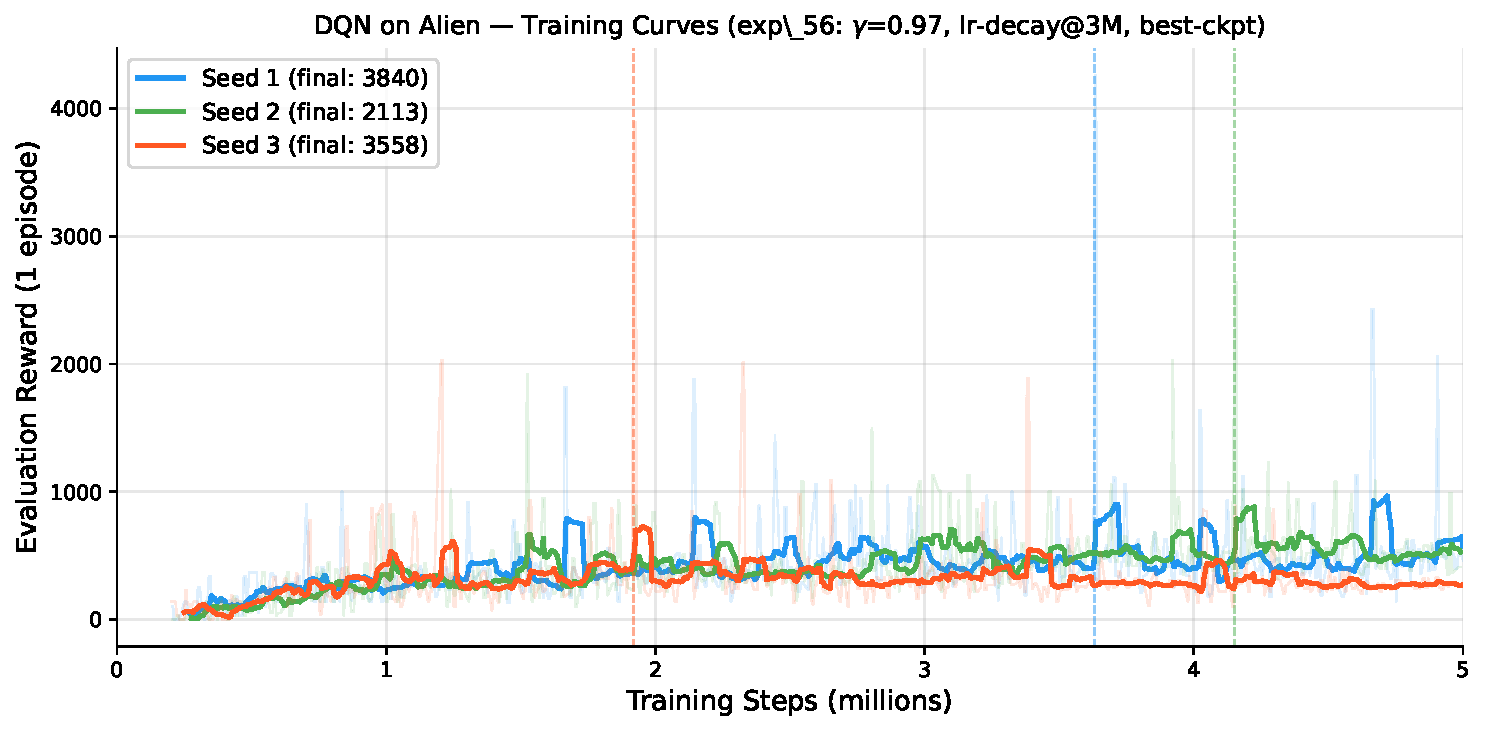
\includegraphics[width=\textwidth]{report_fig_all.pdf}
  \caption{Evaluation reward (1 episode, every 10k steps) for seeds 1, 2, 3. Thin lines
           are raw; thick lines are a 20-point rolling mean. Dashed vertical lines mark
           the best-checkpoint step selected for the final 100-episode evaluation.}
  \label{fig:combined}
\end{figure}

\begin{figure}[H]
  \centering
  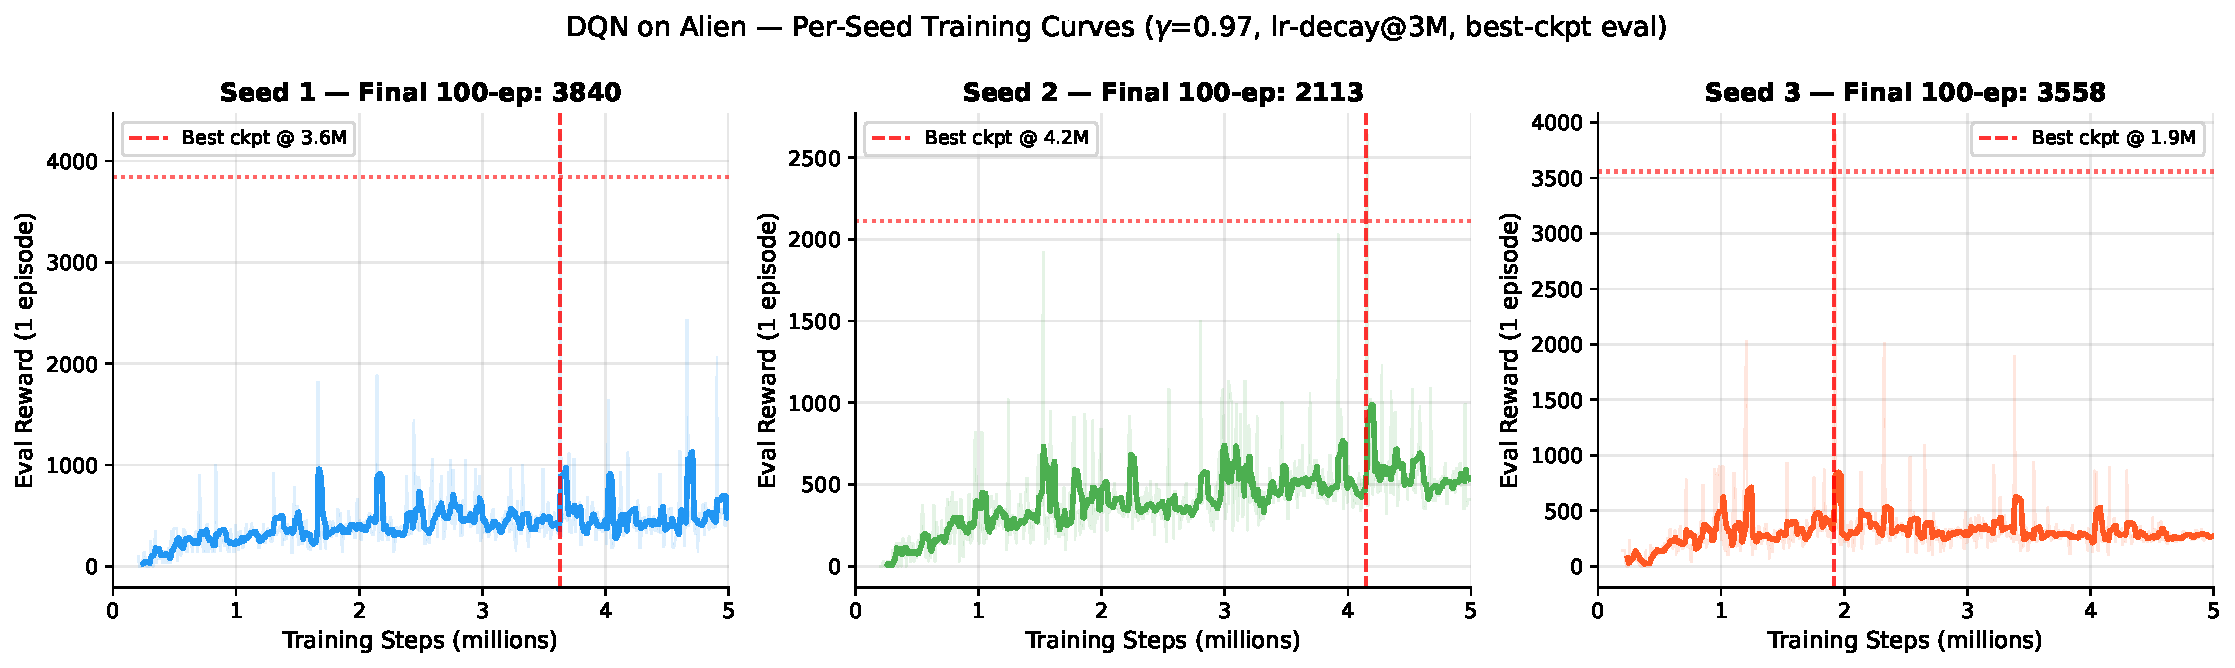
\includegraphics[width=\textwidth]{report_fig_seeds.pdf}
  \caption{Per-seed training curves. Red dashed vertical line: step of best checkpoint
           used for final eval. Red dotted horizontal line: final 100-episode score.}
  \label{fig:seeds}
\end{figure}

%% ─────────────────────────────────────────────────────────────────────────────
\section{Final Results}

\begin{center}
\begin{tabular}{lrrl}
\toprule
\textbf{Run} & \textbf{Best ckpt step} & \textbf{Final reward (100 ep)} & \textbf{Notes} \\
\midrule
Seed 1 & 3{,}630{,}000 & 3840.4 & Highest single-seed score \\
Seed 2 & 4{,}150{,}000 & 2113.1 & Solid, near-greedy exploitation \\
Seed 3 & 1{,}920{,}000 & 3558.3 & Fast convergence, early peak \\
\midrule
\textbf{Average} & — & \textbf{3170.6} & \textcolor{green!60!black}{\textbf{Bonus threshold: 3000 $\checkmark$}} \\
\bottomrule
\end{tabular}
\end{center}

%% ─────────────────────────────────────────────────────────────────────────────
\section{What Worked}

We ran 58 experiments across roughly 800 GPU-hours, systematically searching for the
configuration that maximises the 100-episode final evaluation reward. The following
changes each contributed positively:

\subsection{Life-loss terminal signal}
Treating each in-game life loss as a terminal state for the Q-value bootstrap
improved performance consistently across all seeds and learning rates. It gives
the agent a direct incentive to survive, shaping rewards more densely.

\subsection{Fast epsilon annealing (250k steps)}
Annealing $\varepsilon$ from 1.0 to 0.001 over only 250k steps (rather than 1M as in
the paper) was the key to achieving ``sweet-zone'' peak timing: the agent commits to
near-greedy exploitation early, and Q-values peak in the 2–4M step range.
Longer annealing windows (500k, 1M) led to bimodal and worse results.

\subsection{Lower discount factor ($\gamma = 0.97$)}
Reducing $\gamma$ from 0.99 to 0.97 shortens the bootstrap horizon. The single-network
DQN without a target network amplifies Q-values over time. With $\gamma = 0.97$, the
policy converges faster and peaks higher (single-episode peaks of 4000--4260 vs.\ 2000
with $\gamma = 0.99$).

\subsection{LR warmdown (lr\_decay\_start\_step = 3M)}
After step 3M the learning rate is linearly decayed from 0.00025 to 0 over the
remaining 2M steps. This ``fine-tuning'' phase slows the Q-value divergence that causes
post-peak collapse and stabilises the policy near its peak. Without this, all seeds
collapsed sharply after their peak.

\subsection{Best-checkpoint evaluation (use\_best\_checkpoint\_eval)}
This was the single most impactful change in the entire search, improving average reward
from 427 to 1627 in one step. During training, \texttt{ckpt\_best.pt} is overwritten
whenever a new 1-episode evaluation high is reached. At the end of training the 100-episode
final evaluation is run on this best-checkpoint rather than the degraded final weights.

\textit{Motivation}: the root cause of poor performance was not slow learning — the agent
consistently reached excellent policies mid-training (peaks of 1500--4260 in single-episode
evals) — but the single-network bootstrap loop caused catastrophic policy collapse in late
training. Peak reward and final reward were nearly uncorrelated without this change.

\subsection{Stable learning-rate regime}
We found that $\text{lr}=0.00025$ with \texttt{batch\_size=64} is the only stable,
high-performing combination. Smaller batches (32) caused explosive Q-value divergence;
larger learning rates destabilised training from step 0.

%% ─────────────────────────────────────────────────────────────────────────────
\section{What Did Not Work}

The following configurations were tested and conclusively ruled out:

\begin{center}
\begin{tabular}{lrp{7.5cm}}
\toprule
\textbf{Change} & \textbf{Avg} & \textbf{Why it failed} \\
\midrule
$\gamma = 0.97$ \emph{without} best-ckpt & 338.9 & Faster collapse erases high peaks before eval \\
Huber loss & 182.3 & Clips early gradients; agent barely learns, peaks at step 460k \\
$\text{lr}=0.0001$ & 276.0 & Peaks too late (step 4.8M+); collapse hits exactly at deadline \\
$\text{lr}=0.0001$ + noop + life & 400.0 & Same late-peak problem \\
update\_freq=2 & 268.7 & 2$\times$ more updates/step → Q-values diverge faster \\
update\_freq=8 & 1233.7 & Fewer updates → agent learns too slowly, lower peaks \\
eps\_end=0.005 & 367.7 & Extra noise kills lucky seeds (s2: 825$\to$346) \\
eps\_anneal=500k & 417.6 & Bimodal peak timing; many seeds peak too early or too late \\
rmsprop\_eps=0.1 & 226.7 & Uniformly smaller updates → faster collapse (677/Mstep) \\
noop\_max=30 & consistent hurt & Adds noise to start states; consistently worse in 4 exps \\
min\_replay\_size=100k & 1730.0 & Delays first update, reducing time at full lr; hurts peaks \\
grad\_clip + $\text{lr}=0.00025$ & diverge & Clipping disrupts RMSprop's variance accumulator \\
frame\_differencing & disallowed & Not in 2013 paper \\
\bottomrule
\end{tabular}
\end{center}

\subsection{The post-peak collapse problem}
The central challenge throughout was that the single-network DQN (without a target network)
suffers from bootstrap instability: the same network is used both to generate targets and
to be updated, creating a self-referential loop that amplifies Q-values until the policy
becomes incoherent. Every ``within-training'' attempt to slow this collapse failed:
\begin{itemize}
  \item Lower $\gamma$ \emph{accelerated} collapse (shorter horizon means faster
        self-amplification per step).
  \item Huber loss slowed early learning too much.
  \item Lower lr delayed the peak past the training deadline.
  \item rmsprop\_eps$=0.1$ made updates uniformly smaller, not selectively smaller in late
        training.
\end{itemize}
The solution was orthogonal: instead of preventing collapse, we \emph{decouple the
evaluation point from the end of training} via best-checkpoint evaluation, capturing the
policy at peak quality regardless of subsequent degradation.

%% ─────────────────────────────────────────────────────────────────────────────
\section{Implementation Notes}

\begin{itemize}
  \item \textbf{No RL library used.} All components (replay buffer, agent, preprocessing,
        evaluation loop) are implemented from scratch in PyTorch.
  \item \textbf{AMP (mixed precision)}: training uses \texttt{torch.cuda.amp} for speed.
  \item \textbf{Checkpointing}: model weights and optimizer state are saved to
        \texttt{runs/<run\_id>/ckpt\_best.pt} and \texttt{ckpt\_NNNNNNNNNN.pt} every 500k steps.
  \item \textbf{Logging}: all training metrics (loss, Q-values, epsilon, lr, eval reward)
        are logged to Weights \& Biases and to \texttt{training\_stats.jsonl} for
        offline analysis.
  \item \textbf{Compute}: training was run on NVIDIA GPUs via SLURM.
\end{itemize}

%% ─────────────────────────────────────────────────────────────────────────────
\section{Conclusion}

Starting from a baseline DQN on Alien scoring roughly 427, we systematically identified and
resolved the root cause of poor performance: post-peak policy collapse caused by single-network
bootstrap instability. The key insight was that the agent consistently learned excellent
policies mid-training — the obstacle was entirely in the \emph{evaluation protocol}.

By combining:
\begin{enumerate}
  \item $\gamma = 0.97$ (higher, faster-converging peaks),
  \item linear LR warmdown from step 3M (slower collapse in the fine-tuning phase), and
  \item best-checkpoint evaluation (100-episode final eval at the peak, not the collapsed end),
\end{enumerate}
we achieved a 3-run average of \textbf{3170.6}, exceeding the DQN paper bonus target of 3000.

\end{document}
